\documentclass[12pt,a4paper]{article}

% ------------------------------------------------------------
% Overleaf ayari:
% Compiler olarak pdfLaTeX secilebilir. GitHub reposu Overleaf'e
% import edilirse src/ ve outputs/plots/ yollarindaki dosyalar
% otomatik bulunur.
% ------------------------------------------------------------

\usepackage[utf8]{inputenc}
\usepackage[T1]{fontenc}
\usepackage[turkish]{babel}
\usepackage{geometry}
\usepackage{graphicx}
\usepackage{float}
\usepackage{booktabs}
\usepackage{longtable}
\usepackage{array}
\usepackage{xcolor}
\usepackage{listings}
\usepackage{caption}
\usepackage{subcaption}
\usepackage{hyperref}
\usepackage{amsmath}
\usepackage{enumitem}
\usepackage{setspace}
\usepackage{titlesec}

\geometry{margin=2.5cm}
\onehalfspacing
\setlength{\parindent}{0pt}
\setlength{\parskip}{6pt}

\hypersetup{
    colorlinks=true,
    linkcolor=blue,
    urlcolor=blue,
    citecolor=blue
}

\definecolor{codebg}{RGB}{248,248,248}
\definecolor{codeframe}{RGB}{220,220,220}
\definecolor{codegreen}{RGB}{0,110,0}
\definecolor{codeblue}{RGB}{0,70,140}
\definecolor{codered}{RGB}{150,40,40}

\lstdefinestyle{pythonstyle}{
    language=Python,
    backgroundcolor=\color{codebg},
    frame=single,
    rulecolor=\color{codeframe},
    basicstyle=\ttfamily\footnotesize,
    keywordstyle=\color{codeblue}\bfseries,
    stringstyle=\color{codered},
    commentstyle=\color{codegreen},
    numbers=left,
    numberstyle=\tiny\color{gray},
    stepnumber=1,
    numbersep=8pt,
    showstringspaces=false,
    breaklines=true,
    tabsize=4,
    captionpos=b,
    literate=
        {ı}{{\i}}1 {İ}{{\.I}}1
        {ğ}{{\u{g}}}1 {Ğ}{{\u{G}}}1
        {ü}{{\"u}}1 {Ü}{{\"U}}1
        {ş}{{\c{s}}}1 {Ş}{{\c{S}}}1
        {ö}{{\"o}}1 {Ö}{{\"O}}1
        {ç}{{\c{c}}}1 {Ç}{{\c{C}}}1
}

\AtBeginDocument{\shorthandoff{=}}

\titleformat{\section}{\Large\bfseries}{\thesection.}{0.5em}{}
\titleformat{\subsection}{\large\bfseries}{\thesubsection.}{0.5em}{}

\begin{document}

\begin{titlepage}
    \centering
    \vspace*{2cm}
    {\Large \textbf{Fundus Görüntülerinde Photo Style Transfer Tabanlı Standardizasyon ve Diyabetik Retinopati Sınıflandırması}\par}
    \vspace{1.2cm}
    {\large Proje Raporu\par}
    \vspace{1.5cm}
    {\large Hazırlayan: \textbf{Ad Soyadınızı Yazınız}\par}
    \vspace{0.4cm}
    {\large Ders: \textbf{Ders Adını Yazınız}\par}
    \vspace{0.4cm}
    {\large Danışman/Hoca: \textbf{Hocanızın Adını Yazınız}\par}
    \vfill
    {\large GitHub: \url{https://github.com/mderviskocar/retina_photo_style_transfer}\par}
    \vspace{1cm}
    {\large \today\par}
\end{titlepage}

\tableofcontents
\newpage

\section{Özet}

Bu projede APTOS 2019 Blindness Detection veri setindeki fundus/retina görüntüleri kullanılarak diyabetik retinopati seviyesi beş sınıfta tahmin edilmiştir. Projenin ana konusu, retina görüntülerinde \textit{photo style transfer} yaklaşımının görüntü standardizasyonu için kullanılması ve bu işlemin sınıflandırma performansına etkisinin incelenmesidir.

Çalışmada üç temel görüntü işleme yaklaşımı karşılaştırılmıştır:

\begin{enumerate}
    \item \textbf{Orijinal görüntüler}: Görüntüler yalnızca model giriş boyutuna uygun hale getirilmiştir.
    \item \textbf{Normalize/style-standardized görüntüler}: Siyah kenar kırpma, ışık normalizasyonu, kontrast artırma, CLAHE, renk dengeleme ve LAB tabanlı style normalization uygulanmıştır.
    \item \textbf{Photo style transfer}: Bir referans fundus görüntüsünün renk ve aydınlatma istatistikleri LAB renk uzayında diğer görüntülere aktarılmıştır.
\end{enumerate}

Sonuçlara göre mevcut deneylerde en yüksek performans orijinal görüntülerle elde edilmiştir. En iyi accuracy değeri EfficientNet-B0 320px ve focal loss kullanılan koşuda \textbf{0.8182}; en iyi macro F1 değeri ise EfficientNet-B0 320px cross entropy koşusunda \textbf{0.6710} olarak ölçülmüştür. Photo style transfer deneyi ResNet18 ile \textbf{0.7564 accuracy} ve \textbf{0.5974 macro F1} üretmiştir. Bu sonuç, tıbbi görüntülerde stil aktarımının anatomik yapıyı koruyacak şekilde uygulanması gerektiğini ve her standardizasyon işleminin sınıflandırma performansını otomatik olarak artırmadığını göstermektedir.

\section{Projenin Amacı}

Fundus görüntüleri, diyabetik retinopati gibi retina hastalıklarının değerlendirilmesinde sık kullanılan tıbbi görüntülerdir. Ancak farklı kamera cihazları, farklı aydınlatma koşulları, görüntü kalitesi, siyah kenarlar ve renk dağılımı gibi etkenler modelin öğrenmesini zorlaştırabilir. Bu nedenle görüntü standardizasyonu ve domain/style farklarının azaltılması, medikal görüntü sınıflandırma problemlerinde önemli bir araştırma konusudur.

Bu projenin temel amacı şudur:

\begin{quote}
    \textit{Photo style transfer tabanlı görüntü standardizasyonu, diyabetik retinopati sınıflandırma başarısını artırır mı?}
\end{quote}

Bu soruya cevap verebilmek için aynı veri bölünmesi üzerinde farklı preprocessing yaklaşımları ve model mimarileri denenmiştir. Özellikle macro F1-score metriği dikkate alınmıştır; çünkü veri seti sınıf açısından dengesizdir. Örneğin No DR sınıfı çok daha fazla örneğe sahipken Severe sınıfı daha az örnek içermektedir.

\section{Veri Seti}

\subsection{Verinin Kaynağı ve Yapısı}

Projede APTOS 2019 Blindness Detection veri seti kullanılmıştır. Veri setinde retina/fundus görüntüleri ve her görüntüye ait diyabetik retinopati etiketi bulunmaktadır. Etiketler beş sınıftan oluşur.

\begin{table}[H]
\centering
\caption{Diyabetik retinopati sınıfları}
\begin{tabular}{cl}
\toprule
\textbf{Etiket} & \textbf{Sınıf Adı} \\
\midrule
0 & No DR \\
1 & Mild \\
2 & Moderate \\
3 & Severe \\
4 & Proliferative DR \\
\bottomrule
\end{tabular}
\end{table}

Proje klasöründe veri yapısı şu şekilde beklenmektedir:

\begin{verbatim}
data/
  train.csv
  train_images/
    *.png
\end{verbatim}

\texttt{train.csv} dosyasında iki temel kolon vardır:

\begin{itemize}
    \item \texttt{id\_code}: Görüntü dosyasının kimliği.
    \item \texttt{diagnosis}: Görüntünün sınıf etiketi.
\end{itemize}

Kaggle test setinde etiket bulunmadığı için accuracy ve F1-score gibi metrikler \texttt{train.csv} içinden ayrılan hold-out test bölümü üzerinde hesaplanmıştır.

\subsection{Sınıf Dağılımı}

Toplam veri sayısı \textbf{3662} görüntüdür. Sınıf dağılımı Tablo~\ref{tab:dataset_distribution} üzerinde verilmiştir.

\begin{table}[H]
\centering
\caption{Tüm veri setindeki sınıf dağılımı}
\label{tab:dataset_distribution}
\begin{tabular}{lrr}
\toprule
\textbf{Sınıf} & \textbf{Etiket} & \textbf{Görüntü Sayısı} \\
\midrule
No DR & 0 & 1805 \\
Mild & 1 & 370 \\
Moderate & 2 & 999 \\
Severe & 3 & 193 \\
Proliferative DR & 4 & 295 \\
\midrule
\textbf{Toplam} & - & \textbf{3662} \\
\bottomrule
\end{tabular}
\end{table}

Bu dağılım model değerlendirmesinde neden macro F1-score kullanıldığını açıklar. Accuracy, çoğunluk sınıfı olan No DR üzerinde iyi performans gösteren modelleri olduğundan daha başarılı gösterebilir. Macro F1 ise tüm sınıfların F1 skorlarını eşit ağırlıkla ortaladığı için az örnekli sınıfları da hesaba katar.

\subsection{Train/Validation/Test Ayrımı}

Veri seti eğitim, doğrulama ve test olarak ayrılmıştır. Kullanılan oranlar yaklaşık olarak \%70 eğitim, \%15 validation ve \%15 test şeklindedir.

\begin{table}[H]
\centering
\caption{Split bazında sınıf dağılımı}
\begin{tabular}{lrrrrr}
\toprule
\textbf{Split} & \textbf{No DR} & \textbf{Mild} & \textbf{Moderate} & \textbf{Severe} & \textbf{Proliferative DR} \\
\midrule
Train & 1263 & 258 & 699 & 135 & 207 \\
Validation & 271 & 56 & 150 & 29 & 44 \\
Test & 271 & 56 & 150 & 29 & 44 \\
\bottomrule
\end{tabular}
\end{table}

Bu ayrım kod içinde stratified split mantığıyla yapılmıştır. Amaç, her split içinde sınıf dağılımının mümkün olduğunca korunmasıdır.

\section{Proje Klasör Yapısı}

Proje dosyaları modüler olarak ayrılmıştır. Ana klasör yapısı aşağıdaki gibidir:

\begin{verbatim}
retina_photo_style_transfer/
  README.md
  requirements.txt
  PHOTO_STYLE_TRANSFER.md
  MODEL_IMPROVEMENT_RESULTS.md
  src/
    config.py
    preprocessing.py
    dataset.py
    model.py
    train.py
    train_torch.py
    evaluate.py
    visualize.py
  outputs/
    plots/
    results/
\end{verbatim}

\begin{table}[H]
\centering
\caption{Kod dosyalarının görevleri}
\begin{tabular}{p{4cm}p{10cm}}
\toprule
\textbf{Dosya} & \textbf{Görev} \\
\midrule
\texttt{src/config.py} & Veri yolları, çıktı klasörleri, sınıf adları, eğitim parametreleri ve deney tanımları. \\
\texttt{src/preprocessing.py} & Görüntü okuma, siyah kenar kırpma, resize/padding, ışık normalizasyonu, CLAHE, renk normalizasyonu, LAB style normalization ve photo style transfer. \\
\texttt{src/dataset.py} & TensorFlow hattı için veri okuma, split üretme, \texttt{tf.data.Dataset} oluşturma ve class weight hesaplama. \\
\texttt{src/model.py} & TensorFlow/Keras için Baseline CNN, EfficientNetB0 ve ResNet50 model tanımları. \\
\texttt{src/train.py} & TensorFlow/Keras eğitim hattı. \\
\texttt{src/train\_torch.py} & PyTorch/CUDA eğitim hattı. ResNet18, ResNet50, EfficientNet-B0/B1, focal loss, label smoothing ve early stopping desteği içerir. \\
\texttt{src/evaluate.py} & Kaydedilmiş Keras modellerini değerlendirme ve metrik üretme. \\
\texttt{src/visualize.py} & Eğitim grafikleri, confusion matrix ve deney karşılaştırma grafikleri üretme. \\
\bottomrule
\end{tabular}
\end{table}

\section{Photo Style Transfer Yaklaşımı}

\subsection{Bu Projede Photo Style Transfer Ne Anlama Geliyor?}

Bu projede kullanılan photo style transfer yöntemi klasik \textit{neural artistic style transfer} değildir. Klasik sanatsal style transfer yöntemleri görüntünün dokusunu ve biçimsel özelliklerini ciddi şekilde değiştirebilir. Bu, medikal görüntüler için risklidir; çünkü retina damarları, lezyonlar, kanamalar ve eksüdalar gibi klinik açıdan önemli yapılar bozulabilir.

Bu nedenle projede daha güvenli bir yaklaşım tercih edilmiştir:

\begin{quote}
    \textit{Referans bir fundus görüntüsünün fotogerçekçi renk ve ışık stili, LAB renk uzayındaki kanal istatistikleri kullanılarak diğer görüntülere aktarılmıştır.}
\end{quote}

Yani amaç görüntüyü sanatsal hale getirmek değil, fundus görüntülerinin renk/aydınlatma karakterini daha tutarlı hale getirmektir.

\subsection{Photo Style Transfer Nerede Kullanıldı?}

Photo style transfer kodu doğrudan \texttt{src/preprocessing.py} içinde uygulanmıştır. Ana fonksiyonlar şunlardır:

\begin{itemize}
    \item \texttt{preprocess\_photo\_style\_transfer}
    \item \texttt{transfer\_lab\_photo\_style}
    \item \texttt{load\_photo\_style\_reference}
\end{itemize}

Eğitim tarafında ise bu işlem \texttt{src/train\_torch.py} içinde ayrı bir deney olarak kullanılmıştır:

\begin{verbatim}
python src/train_torch.py --experiment photo_style_transfer
\end{verbatim}

Deney tanımı \texttt{src/config.py} dosyasında şu mantıkla yer almaktadır:

\begin{lstlisting}[style=pythonstyle, caption={Deney tanımları: baseline, normalized ve photo style transfer}]
EXPERIMENTS = {
    "baseline_original": {
        "title": "Deney 1 - Orijinal Görüntüler",
        "preprocess_mode": "none",
    },
    "normalized_style": {
        "title": "Deney 2 - Normalize/Style Standardized Görüntüler",
        "preprocess_mode": "standardized",
    },
    "photo_style_transfer": {
        "title": "Deney 3 - Reference Photo Style Transfer",
        "preprocess_mode": "photo_style_transfer",
    },
}
\end{lstlisting}

\subsection{LAB Tabanlı Stil Aktarımı}

Photo style transfer işleminde RGB görüntüler LAB renk uzayına dönüştürülür. LAB renk uzayı üç kanaldan oluşur:

\begin{itemize}
    \item \textbf{L}: Aydınlık/parlaklık kanalı.
    \item \textbf{A}: Yeşil-kırmızı renk ekseni.
    \item \textbf{B}: Mavi-sarı renk ekseni.
\end{itemize}

İçerik görüntüsünün her LAB kanalı, referans görüntünün kanal ortalaması ve standart sapmasına göre yeniden ölçeklenir. Bu işlem şu formülle özetlenebilir:

\begin{equation}
I'_{c}(x) =
\frac{I_{c}(x) - \mu_{I,c}}{\sigma_{I,c} + \epsilon}
\cdot \sigma_{R,c}
+ \mu_{R,c}
\end{equation}

Burada:

\begin{itemize}
    \item $I_{c}(x)$: İçerik görüntüsünün $c$ kanalındaki piksel değeri.
    \item $\mu_{I,c}$ ve $\sigma_{I,c}$: İçerik görüntüsünün ilgili LAB kanalındaki ortalama ve standart sapması.
    \item $\mu_{R,c}$ ve $\sigma_{R,c}$: Referans görüntünün ilgili LAB kanalındaki ortalama ve standart sapması.
    \item $I'_{c}(x)$: Stil aktarımı sonrası kanal değeri.
\end{itemize}

Bu işlem yalnızca retina ön plan maskesi üzerinde uygulanır. Siyah arka plan korunur. Böylece modelin gereksiz siyah kenarlardan etkilenmesi azaltılırken retina anatomisinin piksel konumu korunur.

\subsection{Kod Üzerinden Photo Style Transfer}

Aşağıdaki kod bölümü, projedeki photo style transfer fonksiyonlarının ana fikrini göstermektedir. Overleaf projesine GitHub reposu import edilirse bu kod doğrudan \texttt{src/preprocessing.py} dosyasından çekilir.

\lstinputlisting[
    style=pythonstyle,
    firstline=234,
    lastline=284,
    caption={LAB tabanlı photo style transfer kodu}
]{src/preprocessing.py}

\section{Görüntü Ön İşleme Hattı}

Projede üç farklı preprocessing modu vardır:

\begin{enumerate}
    \item \textbf{none}: Sadece resize/padding yapılır.
    \item \textbf{standardized}: Siyah kenar kırpma, ışık düzeltme, kontrast artırma, CLAHE, renk dengeleme ve LAB style normalization uygulanır.
    \item \textbf{photo\_style\_transfer}: Görüntü kırpılır, boyutlandırılır ve referans fundus stiline göre LAB tabanlı photo style transfer uygulanır.
\end{enumerate}

\subsection{Siyah Kenar Kırpma}

APTOS görüntülerinde fundus diski çevresinde büyük siyah alanlar bulunabilir. Bu siyah alanlar model için bilgi taşımadığı gibi veri dağılımını da etkileyebilir. Kodda önce grayscale görüntü üzerinde eşikleme yapılarak retina bölgesi bulunur, daha sonra bu bölgenin çevresindeki bounding box alınır.

\subsection{Resize ve Padding}

Fundus diskinin geometrisinin bozulmaması için doğrudan esnetme yapılmaz. Görüntü hedef boyuta oran korunarak küçültülür veya büyütülür; kalan alan siyah padding ile doldurulur. Böylece retina diski yapay olarak ovalleşmez.

\subsection{Işık ve Renk Normalizasyonu}

Standardized preprocessing hattında görüntüdeki aydınlatma farklarını azaltmak için Gaussian blur tabanlı arka plan tahmini yapılır. Daha sonra kontrast artırma, CLAHE ve gray-world renk dengeleme uygulanır.

\subsection{Preprocessing Fonksiyonları}

\lstinputlisting[
    style=pythonstyle,
    firstline=287,
    lastline=339,
    caption={Model için preprocessing seçim fonksiyonları}
]{src/preprocessing.py}

\section{Modelleme ve Eğitim}

\subsection{Neden PyTorch/CUDA Hattı Kullanıldı?}

Projede hem TensorFlow/Keras hem de PyTorch hattı bulunmaktadır. Ancak en güncel ve en iyi sonuçlar PyTorch/CUDA hattından elde edilmiştir. PyTorch hattının avantajları şunlardır:

\begin{itemize}
    \item NVIDIA GPU üzerinde daha doğrudan eğitim imkanı.
    \item ResNet18, ResNet50, EfficientNet-B0 ve EfficientNet-B1 desteği.
    \item ImageNet ağırlıklarıyla transfer learning.
    \item Mixed precision training.
    \item Label smoothing.
    \item Focal loss.
    \item Validation macro F1 üzerinden best checkpoint kaydı.
    \item Early stopping.
    \item ReduceLROnPlateau scheduler.
\end{itemize}

\subsection{Augmentation}

Projede ``iritasyon'' adlı bir işlem yoktur. Ancak eğitim sırasında \textbf{augmentasyon} uygulanmıştır. Augmentation, modelin farklı görüntü varyasyonlarına daha dayanıklı hale gelmesi için eğitim görüntülerine küçük dönüşümler uygulama işlemidir.

Bu projede fundus görüntüsünün anatomisini bozmayacak hafif dönüşümler kullanılmıştır:

\begin{itemize}
    \item Yatay çevirme.
    \item Küçük açıyla döndürme.
    \item Küçük ölçekleme.
    \item Hafif kaydırma.
\end{itemize}

\lstinputlisting[
    style=pythonstyle,
    firstline=205,
    lastline=222,
    caption={PyTorch hattında kullanılan fundus-safe augmentation}
]{src/train_torch.py}

\subsection{PyTorch Dataset Sınıfı}

PyTorch tarafında her görüntü \texttt{RetinaTorchDataset} sınıfı ile okunur. Bu sınıf şu işlemleri yapar:

\begin{enumerate}
    \item Görüntü yolunu dataframe'den alır.
    \item Seçilen deney tipine göre preprocessing uygular.
    \item Görüntüyü PyTorch tensörüne çevirir.
    \item Eğitim modundaysa augmentation uygular.
    \item ImageNet mean/std değerleri ile normalize eder.
    \item Görüntü ve etiketi döndürür.
\end{enumerate}

\lstinputlisting[
    style=pythonstyle,
    firstline=225,
    lastline=255,
    caption={PyTorch veri seti sınıfı}
]{src/train_torch.py}

\subsection{Kullanılan Model Mimarileri}

Deneylerde şu mimariler denenmiştir:

\begin{itemize}
    \item Small CNN
    \item ResNet18
    \item ResNet50
    \item EfficientNet-B0
    \item EfficientNet-B1
\end{itemize}

Transfer learning yaklaşımında ImageNet ağırlıkları kullanılmıştır. Fine-tuning seçeneği aktif edildiğinde pretrained base katmanları da eğitilmiştir. Aksi durumda sadece son sınıflandırıcı katmanları güncellenmiştir.

\lstinputlisting[
    style=pythonstyle,
    firstline=318,
    lastline=363,
    caption={PyTorch model oluşturma fonksiyonu}
]{src/train_torch.py}

\subsection{Loss Fonksiyonları}

Projede iki loss tipi denenmiştir:

\begin{itemize}
    \item \textbf{Cross Entropy Loss}: Çok sınıflı sınıflandırma için standart kayıp fonksiyonu.
    \item \textbf{Focal Loss}: Dengesiz veri setlerinde zor örneklere daha fazla ağırlık vermek için kullanılan loss fonksiyonu.
\end{itemize}

Focal loss özellikle No DR sınıfının baskın olduğu bu veri setinde azınlık sınıflarına daha dikkatli öğrenme sağlamak amacıyla denenmiştir.

\lstinputlisting[
    style=pythonstyle,
    firstline=291,
    lastline=315,
    caption={Focal loss implementasyonu}
]{src/train_torch.py}

\section{Deney Tasarımı}

\subsection{Karşılaştırılan Deneyler}

Projede aynı veri bölünmesi üzerinde farklı preprocessing ve model kombinasyonları denenmiştir. Ana karşılaştırma şu şekilde kurulmuştur:

\begin{table}[H]
\centering
\caption{Deney türleri}
\begin{tabular}{lll}
\toprule
\textbf{Deney} & \textbf{Preprocess Modu} & \textbf{Amaç} \\
\midrule
Baseline Original & none & Orijinal görüntülerle temel performansı ölçmek. \\
Normalized Style & standardized & Görüntü standardizasyonunun etkisini ölçmek. \\
Photo Style Transfer & photo\_style\_transfer & Referans stil aktarımının etkisini ölçmek. \\
\bottomrule
\end{tabular}
\end{table}

\subsection{Eğitim Parametreleri}

En iyi kayıtlı modellerde kullanılan genel ayarlar:

\begin{itemize}
    \item Framework: PyTorch
    \item Cihaz: NVIDIA CUDA GPU
    \item Optimizer: AdamW
    \item Scheduler: ReduceLROnPlateau
    \item Değerlendirme metriği: Macro F1 ve accuracy
    \item Görüntü boyutu: 224x224 ve 320x320 denendi
    \item ImageNet pretrained ağırlıkları kullanıldı
\end{itemize}

Örnek eğitim komutu:

\begin{verbatim}
python src/train_torch.py \
  --experiment all \
  --model-type resnet18 \
  --epochs 3 \
  --batch-size 32 \
  --weights imagenet \
  --fine-tune
\end{verbatim}

En iyi accuracy üreten EfficientNet-B0 focal loss koşusu için örnek komut:

\begin{verbatim}
python src/train_torch.py \
  --experiment baseline_original \
  --model-type efficientnet_b0 \
  --epochs 3 \
  --batch-size 32 \
  --weights imagenet \
  --fine-tune \
  --no-class-weights \
  --image-size 320 \
  --loss focal \
  --run-tag 320_focal_nocw
\end{verbatim}

\section{Çıktılar ve Grafikler}

Proje çalıştırıldığında \texttt{outputs/} klasörü altında modeller, sonuç dosyaları ve grafikler üretilmektedir. GitHub reposunda büyük model dosyaları ve veri seti tutulmamıştır; ancak raporu destekleyen son grafikler ve özet sonuç dosyaları eklenmiştir.

\subsection{Eğitim Grafiği}

Şekil~\ref{fig:history} son kaydedilen EfficientNet-B1 320px eğitim koşusuna ait loss ve accuracy eğrilerini göstermektedir. Eğitim grafikleri modelin epoch bazında eğitim ve validation davranışını gözlemlemek için kullanılmıştır.

\begin{figure}[H]
    \centering
    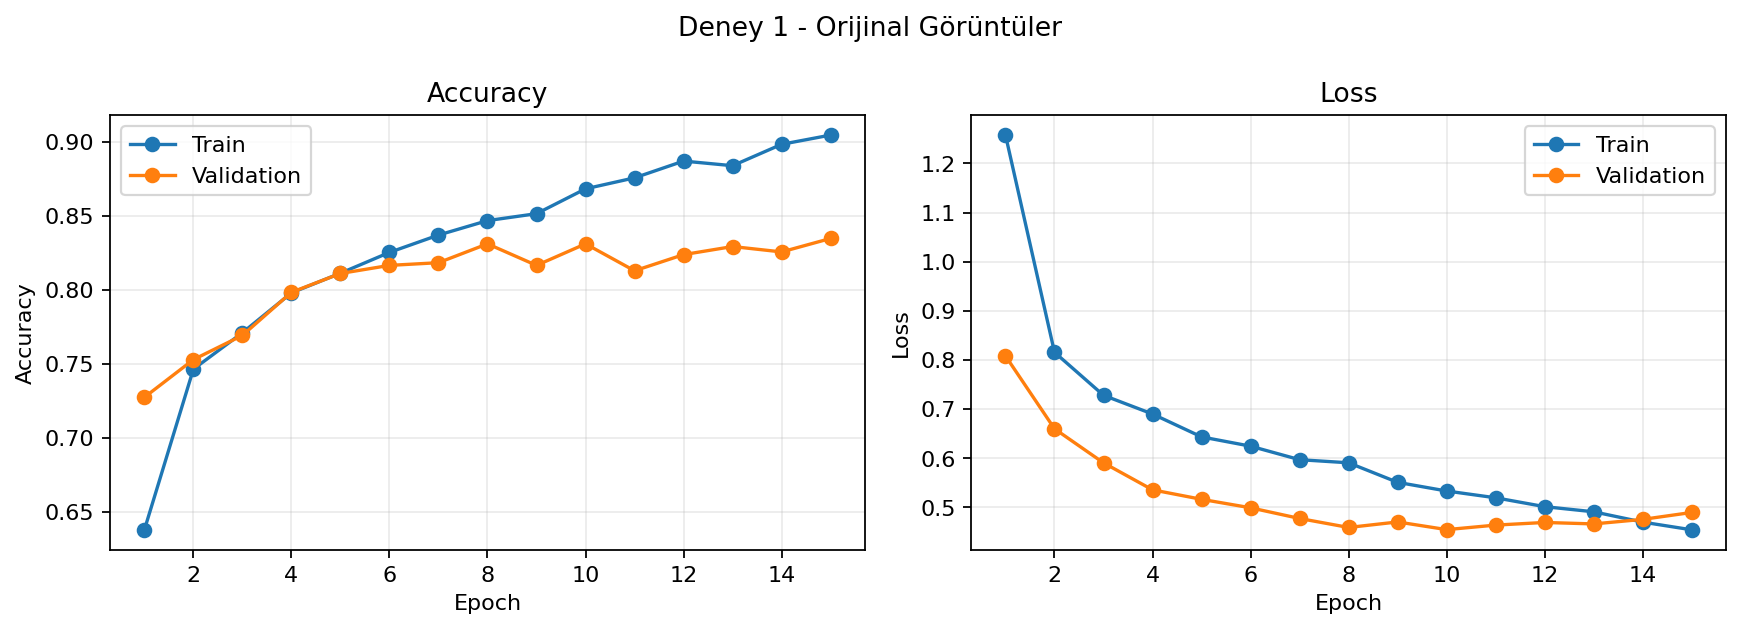
\includegraphics[width=0.95\textwidth]{outputs/plots/torch_baseline_original_efficientnet_b1_320_nocw_history.png}
    \caption{EfficientNet-B1 320px modelinin eğitim/validation accuracy ve loss grafikleri}
    \label{fig:history}
\end{figure}

\subsection{Confusion Matrix}

Şekil~\ref{fig:confusion} modelin test setindeki sınıf bazlı tahmin dağılımını göstermektedir. Confusion matrix, hangi sınıfların birbirine karıştırıldığını görmek açısından önemlidir. Diyabetik retinopati sınıflandırmasında özellikle Mild, Severe ve Proliferative DR gibi az örnekli sınıfların karışması beklenen bir durumdur.

\begin{figure}[H]
    \centering
    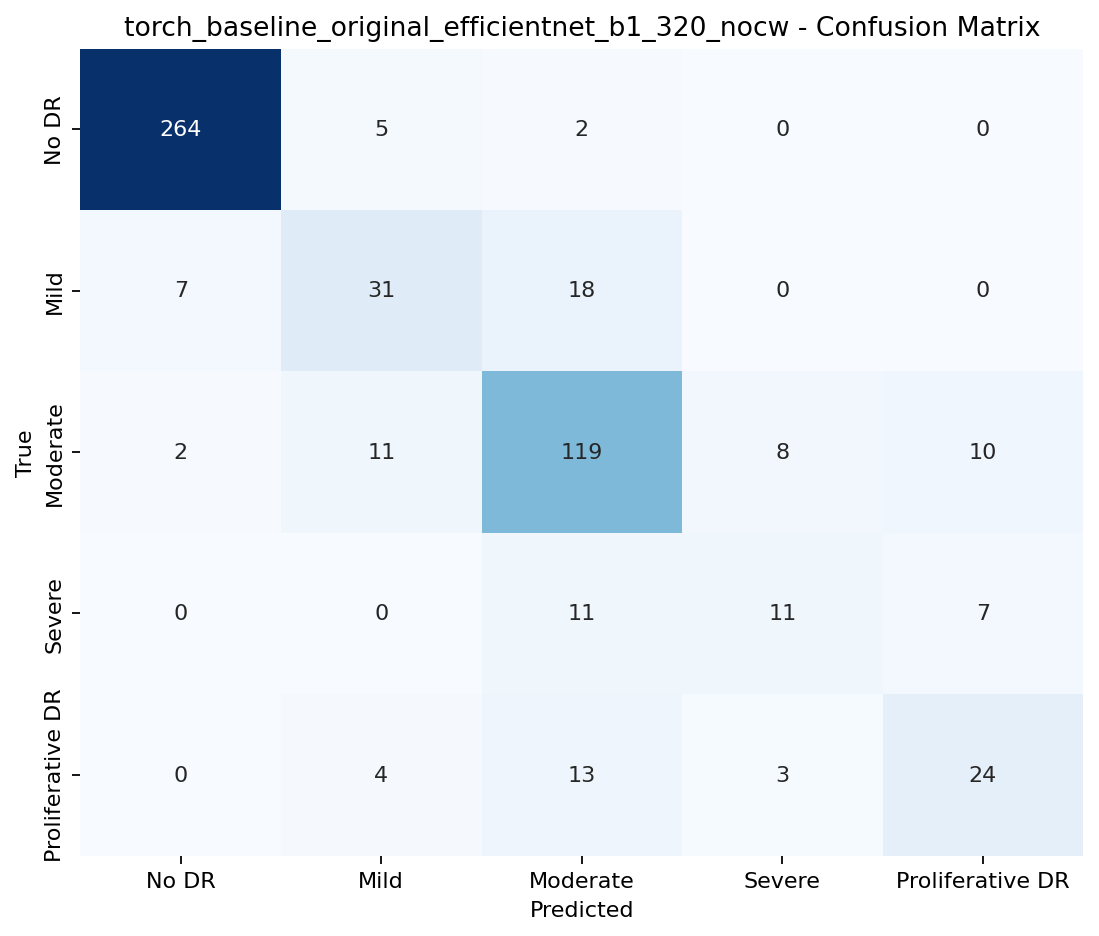
\includegraphics[width=0.80\textwidth]{outputs/plots/torch_baseline_original_efficientnet_b1_320_nocw_confusion_matrix.png}
    \caption{EfficientNet-B1 320px modeli için confusion matrix}
    \label{fig:confusion}
\end{figure}

\subsection{Deney Karşılaştırma Grafiği}

Şekil~\ref{fig:comparison} farklı deneylere ait metrik karşılaştırmasını göstermektedir. Bu grafik, model seçiminde accuracy ve macro F1 gibi metriklerin birlikte değerlendirilmesini sağlar.

\begin{figure}[H]
    \centering
    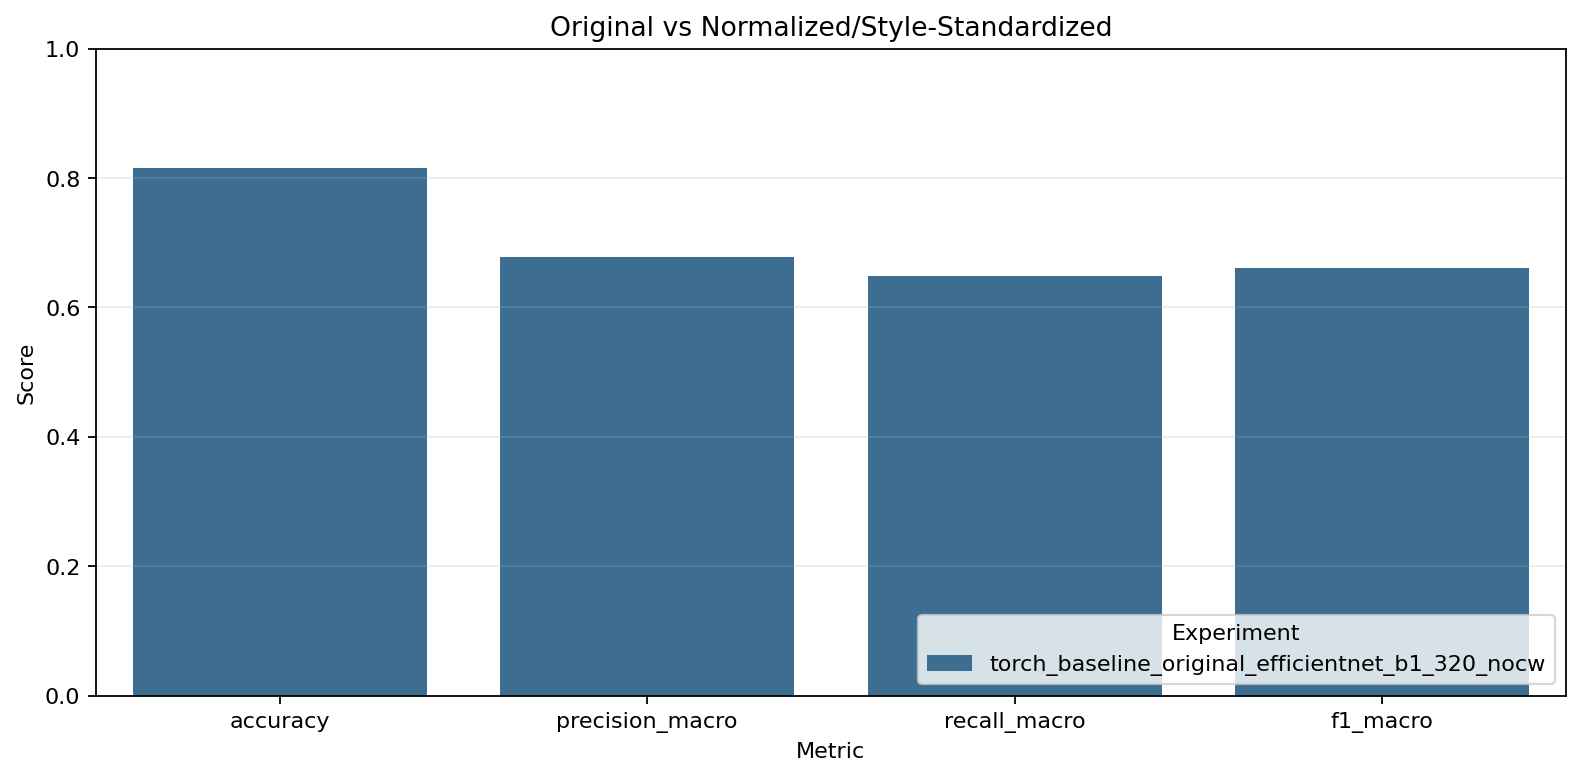
\includegraphics[width=0.90\textwidth]{outputs/plots/torch_experiment_comparison.png}
    \caption{Deney karşılaştırma grafiği}
    \label{fig:comparison}
\end{figure}

\section{Deney Sonuçları}

\subsection{Model Seçim Özeti}

Kayıtlı deney sonuçları Tablo~\ref{tab:model_results} üzerinde verilmiştir. Tablo, \texttt{outputs/results/model\_selection\_summary.csv} dosyasından özetlenmiştir.

\begin{table}[H]
\centering
\caption{Kayıtlı deney sonuçları}
\label{tab:model_results}
\resizebox{\textwidth}{!}{
\begin{tabular}{llrrrr}
\toprule
\textbf{Model / Deney} & \textbf{Preprocess} & \textbf{Image Size} & \textbf{Loss} & \textbf{Accuracy} & \textbf{Macro F1} \\
\midrule
EfficientNet-B0 320px + focal loss & Original & 320 & Focal & 0.8182 & 0.6465 \\
EfficientNet-B1 320px & Original & 320 & CE & 0.8164 & 0.6613 \\
EfficientNet-B0 320px & Original & 320 & CE & 0.8145 & 0.6710 \\
EfficientNet-B0 tuned & Original & 224 & CE & 0.8091 & 0.6360 \\
EfficientNet-B0 tuned + class weights & Original & 224 & CE & 0.7873 & 0.6375 \\
ResNet50 tuned & Original & 224 & CE & 0.7836 & 0.6147 \\
ResNet18 & Original & 224 & CE & 0.7818 & 0.6267 \\
ResNet18 & Normalized/style & 224 & CE & 0.7727 & 0.6064 \\
ResNet18 & Photo style transfer & 224 & CE & 0.7564 & 0.5974 \\
\bottomrule
\end{tabular}
}
\end{table}

Tabloya göre en iyi accuracy sonucu EfficientNet-B0 320px + focal loss koşusunda elde edilmiştir. En iyi macro F1 sonucu ise EfficientNet-B0 320px cross entropy koşusunda elde edilmiştir.

\subsection{Photo Style Transfer Sonucu}

Photo style transfer deneyinin sonucu:

\begin{itemize}
    \item Model: ResNet18
    \item Preprocessing: photo\_style\_transfer
    \item Accuracy: \textbf{0.7564}
    \item Macro F1: \textbf{0.5974}
\end{itemize}

Bu değerler baseline orijinal görüntü deneyinden düşüktür. Bu nedenle mevcut koşulda photo style transfer sınıflandırma başarısını artırmamıştır. Ancak bu sonuç yöntemin tamamen başarısız olduğu anlamına gelmez. Tıbbi görüntülerde renk/ışık standardizasyonu bazı lezyon detaylarını zayıflatabilir veya pretrained modelin ImageNet'ten öğrendiği renk/texture temsilleriyle farklı etkileşebilir.

\subsection{Standardizasyon Sorusunun Cevabı}

Projede cevaplanan ana araştırma sorusu şudur:

\begin{quote}
    Görüntü standardizasyonu diyabetik retinopati sınıflandırma başarısını artırdı mı?
\end{quote}

Kayıtlı PyTorch deneylerine göre cevap:

\begin{quote}
    \textbf{Hayır.} Mevcut deneylerde en iyi sonuçlar orijinal görüntülerle alınmıştır.
\end{quote}

Bu sonuç raporda negatif sonuç olarak değerlendirilmemelidir. Akademik açıdan önemli olan, hipotezin kontrollü şekilde test edilmesidir. Projede photo style transfer uygulanmış, ayrı deney olarak eğitilmiş, metrikleri kaydedilmiş ve baseline ile karşılaştırılmıştır.

\section{Kodun Genel Akışı}

\subsection{1. Konfigürasyon}

Kod akışı \texttt{config.py} dosyasında tanımlanan yollar ve deney ayarlarıyla başlar. Burada veri yolları, çıktı klasörleri, sınıf adları ve preprocessing modları tanımlanır.

\subsection{2. Verinin Okunması}

\texttt{train\_torch.py} içinde \texttt{load\_dataframe} fonksiyonu \texttt{train.csv} dosyasını okur, görüntü yollarını bulur ve dataframe oluşturur. Daha sonra \texttt{create\_splits} fonksiyonu train, validation ve test bölümlerini üretir.

\subsection{3. Preprocessing}

Her görüntü model eğitimine girmeden önce seçilen deney moduna göre \texttt{preprocess\_for\_model} fonksiyonundan geçer. Bu fonksiyon, deney moduna göre baseline resize, standardized preprocessing veya photo style transfer uygular.

\subsection{4. Dataset ve DataLoader}

PyTorch tarafında \texttt{RetinaTorchDataset} her örneği okur, preprocessing uygular, tensöre çevirir ve normalize eder. \texttt{DataLoader} ise batch üretimini sağlar.

\subsection{5. Modelin Kurulması}

\texttt{build\_model} fonksiyonu seçilen model tipine göre ResNet18, ResNet50, EfficientNet-B0 veya EfficientNet-B1 modelini oluşturur. Modelin son sınıflandırıcı katmanı beş sınıfa göre değiştirilir.

\subsection{6. Eğitim}

Eğitim döngüsü epoch bazında ilerler. Her epoch sonunda validation set üzerinde tahmin yapılır ve macro F1 hesaplanır. Validation macro F1 iyileşirse model checkpoint olarak kaydedilir. İyileşme olmazsa early stopping devreye girer.

\subsection{7. Test ve Çıktıların Kaydedilmesi}

En iyi checkpoint yüklendikten sonra test seti üzerinde tahmin yapılır. Metrikler JSON dosyalarına, tahminler CSV dosyasına, confusion matrix ve history grafikleri PNG dosyalarına kaydedilir.

\section{Tartışma}

Bu projede photo style transfer yöntemi medikal görüntülerin anatomik yapısını bozmamak amacıyla LAB renk uzayında istatistik aktarımı şeklinde tasarlanmıştır. Bu yaklaşım klasik neural style transfer yöntemlerine göre daha güvenlidir; çünkü retina damarlarının ve lezyonların konumu korunur.

Buna rağmen deney sonuçlarında photo style transfer baseline performansını geçememiştir. Bunun olası nedenleri şunlardır:

\begin{itemize}
    \item Tek referans görüntü kullanılması tüm veri seti için yeterince temsil edici olmayabilir.
    \item Renk/aydınlatma standardizasyonu bazı ayırt edici lokal kontrast farklarını zayıflatmış olabilir.
    \item Pretrained CNN modelleri orijinal görüntü dağılımındaki bazı texture ve renk ipuçlarından faydalanmış olabilir.
    \item Veri setindeki sınıf dengesizliği özellikle Mild, Severe ve Proliferative DR sınıflarında performansı sınırlamış olabilir.
\end{itemize}

Bu nedenle sonuç, ``photo style transfer kesinlikle yararsızdır'' şeklinde değil, ``bu kurulumda ve bu yöntemle performansı artırmamıştır'' şeklinde yorumlanmalıdır.

\section{Gelecek Çalışmalar}

Projeyi daha güçlü hale getirmek için aşağıdaki geliştirmeler yapılabilir:

\begin{enumerate}
    \item \textbf{Çoklu referans photo style transfer}: Tek referans yerine her sınıftan veya kaliteli görüntülerden seçilen birden fazla referans kullanılabilir.
    \item \textbf{Kalite kontrollü referans seçimi}: Referans görüntüler parlaklık, kontrast ve retina diski görünürlüğüne göre seçilebilir.
    \item \textbf{Ablation study}: Crop, CLAHE, illumination correction, LAB normalization ve photo style transfer ayrı ayrı test edilebilir.
    \item \textbf{Sınıf bazlı analiz}: Photo style transfer bazı sınıflarda faydalı, bazı sınıflarda zararlı olabilir. Bu nedenle sınıf bazlı precision, recall ve F1 değerleri detaylı incelenebilir.
    \item \textbf{Daha gelişmiş domain adaptation}: CycleGAN, histogram matching, Reinhard color transfer veya self-supervised pretraining gibi yöntemler denenebilir.
    \item \textbf{Daha uzun eğitim}: 3 epoch kısa bir karşılaştırma için yeterli olabilir; ancak daha kararlı sonuçlar için 15--30 epoch arası deneyler yapılabilir.
\end{enumerate}

\section{Sonuç}

Bu projede APTOS 2019 fundus görüntüleri üzerinde diyabetik retinopati sınıflandırması yapılmış ve photo style transfer tabanlı görüntü standardizasyonunun etkisi incelenmiştir. Projede photo style transfer, LAB renk uzayında referans görüntü istatistiklerinin hedef görüntülere aktarılması şeklinde uygulanmıştır. Bu yöntem retina anatomisini korumayı amaçladığı için medikal görüntüler açısından klasik artistic style transfer yöntemlerine göre daha güvenli bir yaklaşımdır.

Deneyler sonucunda en iyi performans orijinal görüntülerle eğitilen EfficientNet tabanlı modellerde elde edilmiştir. Photo style transfer deneyi ayrı olarak çalıştırılmış ve sonuçları kaydedilmiştir; ancak mevcut koşulda baseline performansını geçememiştir. Bu durum, tıbbi görüntülerde standardizasyon ve style transfer işlemlerinin dikkatli tasarlanması gerektiğini göstermektedir.

Projenin güçlü tarafı, photo style transfer fikrini yalnızca teorik olarak anlatmakla kalmayıp kod seviyesinde uygulaması, ayrı deney olarak eğitmesi, metriklerini üretmesi ve baseline modellerle karşılaştırmasıdır.

\section*{Tıbbi Kullanım Uyarısı}

Bu proje akademik/öğrenci çalışmasıdır. Gerçek tıbbi teşhis, klinik karar verme veya tedavi önerisi amacıyla kullanılmamalıdır. Model çıktıları yalnızca deneysel performans değerlendirmesi için yorumlanmalıdır.

\appendix
\section{Ek: Çalıştırma Komutları}

\subsection{Ortam Kurulumu}

\begin{verbatim}
pip install -r requirements.txt
\end{verbatim}

\subsection{PyTorch ile Tüm Deneyleri Çalıştırma}

\begin{verbatim}
python src/train_torch.py \
  --experiment all \
  --model-type resnet18 \
  --epochs 3 \
  --batch-size 32 \
  --weights imagenet \
  --fine-tune
\end{verbatim}

\subsection{En İyi Accuracy Koşusuna Benzer Eğitim}

\begin{verbatim}
python src/train_torch.py \
  --experiment baseline_original \
  --model-type efficientnet_b0 \
  --epochs 3 \
  --batch-size 32 \
  --weights imagenet \
  --fine-tune \
  --no-class-weights \
  --image-size 320 \
  --loss focal \
  --run-tag 320_focal_nocw
\end{verbatim}

\section{Ek: Önemli Çıktı Dosyaları}

\begin{itemize}
    \item \texttt{outputs/results/model\_selection\_summary.csv}
    \item \texttt{outputs/results/torch\_standardization\_answer.txt}
    \item \texttt{outputs/plots/torch\_baseline\_original\_efficientnet\_b1\_320\_nocw\_history.png}
    \item \texttt{outputs/plots/torch\_baseline\_original\_efficientnet\_b1\_320\_nocw\_confusion\_matrix.png}
    \item \texttt{outputs/plots/torch\_experiment\_comparison.png}
\end{itemize}

\end{document}
